
\documentclass[a4paper, 11pt]{article}
\usepackage[polish]{babel}
\usepackage[T1]{fontenc}
\usepackage[utf8]{inputenc}
\usepackage{hyperref}
\usepackage{array}
\usepackage{amssymb}
\usepackage{amsmath}
\hypersetup{
    colorlinks,
    citecolor=black,
    filecolor=black,
    linkcolor=black,
    urlcolor=black
}
\usepackage{graphicx}

\usepackage{tikz}
\usetikzlibrary{fit,arrows,matrix,positioning, calc, shapes.gates.logic.IEC, shapes.gates.logic.US,arrows,arrows.meta}
\tikzstyle{branch}=[fill,shape=circle,minimum size=3pt,inner sep=0pt]

\title{%
        % \vspace{-3.5cm}
       \large Sprawozdanie Laboratorium PTC \\
       \huge Układy Sekwencyjne 2}

\author{Stanisław Fiedler 160250, L1}
\date{LAB 4, 19 listopada 2024}

\begin{document}

\maketitle
%\tableofcontents

\section{Licznik modulo 12}\label{sec:licznik_modulo_} % (fold)

Zaprojektuj asynchroniczny licznik modulo 12 wykorzystując przerzutniki T korzystając ze
skracania licznika. Zasymuluj układ wykorzystując Logisim.



W liczniku z poprzedniego zadania wydłuż czas trwania sygnału zerującego przerzutniki, tak
aby trwał on połowę cyklu zegara.

\begin{center}
	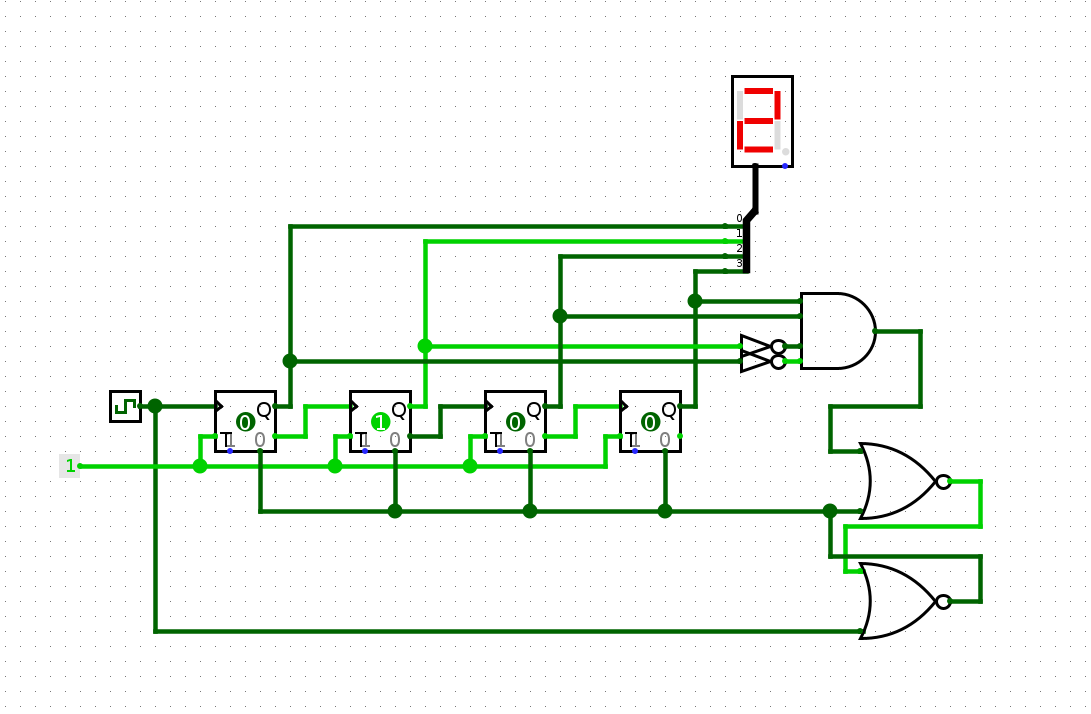
\includegraphics[scale=0.35]{images/licznik.png}
\end{center}
% section Licznik modulo 12 (end)

\end{document}
